\documentclass{article}
\usepackage[a4paper, portrait, margin=1cm, bottom=2cm]{geometry}
\usepackage[fleqn]{amsmath}
\usepackage{graphicx}
\usepackage{fontspec}
\usepackage{indentfirst}

\setmainfont[Ligatures=TeX]{Linux Libertine}
\graphicspath{./graphics/}

\title{Информационные технологии. Лекция 09. Intersection management. ACAS}
\author{Студент группы 2305 Макурин Александр}
\date{17 апреля 2023}
\begin{document}
\maketitle
По сути — задача пересечения перекрёстка. Необходимо оптимально пересечь перекрёсток.

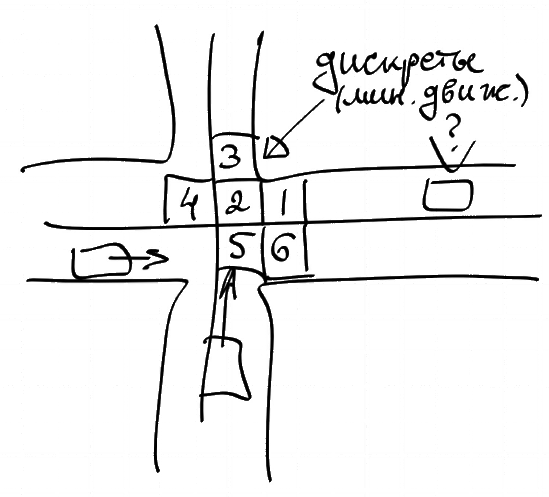
\includegraphics[width=0.6\textwidth]{graphics/pic01.png}

$R = \cup R_S$

$R_s = \{r_i\}$

$R_l \cap R_R$ — зона перекрёстка.

$S_{e_i} = \{r_i\} = \{i : \{r_i\}\}$ — множество участков дороги, которые хочет посетить $e_i$.

Интересуют: $t = 0 : r_0$ и $t = T : r_T$.

\begin{tabular}{|c|c|c|c|c|}
    \hline
    1     & 2     & 3     & 4     & 5     \\
    \hline
    $r_1$ & $r_2$ & $r_3$ & $r_4$ & $r_5$ \\
    \hline
\end{tabular} $V > 1$

Как выбрать дискретное расстояние ($r_i$)?

$V = \begin{cases} 0 \\ 1 \end{cases}$

В качестве одного из вариантов можно взять за $|r_i|$ минимальный тормозной путь.

\subsubsection*{Граф выбора пути:}
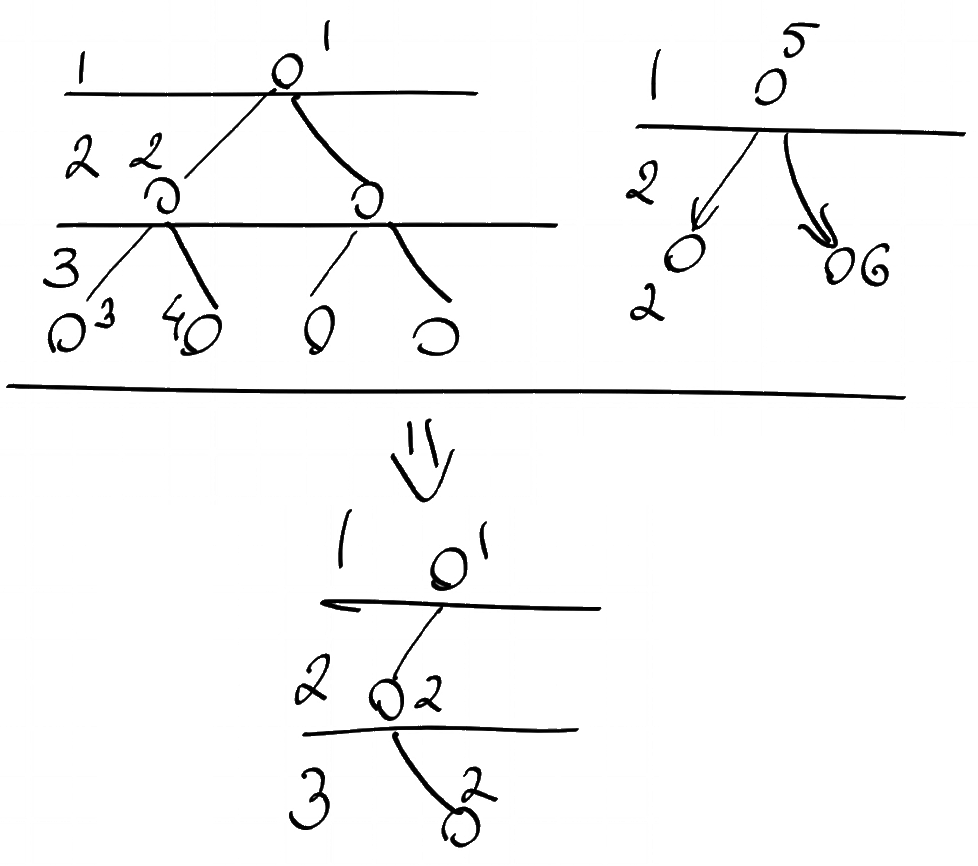
\includegraphics[width=0.5\textwidth]{graphics/pic02.png}

Две машины $\rightarrow$ коллизия (столкновение). Коллизии бывают:
\begin{itemize}
    \item поворотные 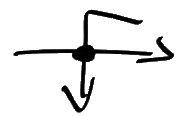
\includegraphics[width=0.1\textwidth]{graphics/pic03.png}
    \item перестроечные 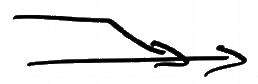
\includegraphics[width=0.1\textwidth]{graphics/pic04.png}
    \item встречные 
\includegraphics[width=0.1\textwidth]{graphics/pic05.png}
    \item слияния (полосы сливаются в одну) 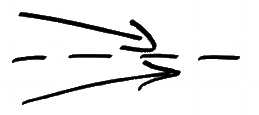
\includegraphics[width=0.1\textwidth]{graphics/pic06.png}
\end{itemize}

Если в одном месте в одно время находится два объекта (автомобиля) (происходит коллизия), то граф пути надо перестроить.

Решение коллизии — один тормозит. Проблема — работает только для одного.

Изменяемые параметры: $V$ — скорость. За счёт них решается задача оптимизации.

$V_{e_i} \rightarrow max \Leftrightarrow T \rightarrow min = T^* \Rightarrow V_{e_i}^{\text{идеал}}$ ($T \rightarrow min$ в идеальных условиях, $T^*$ — время проезда в идеальных условиях).

$a \leq 1$ — ускорение.

\section*{Более сложный перекрёсток}

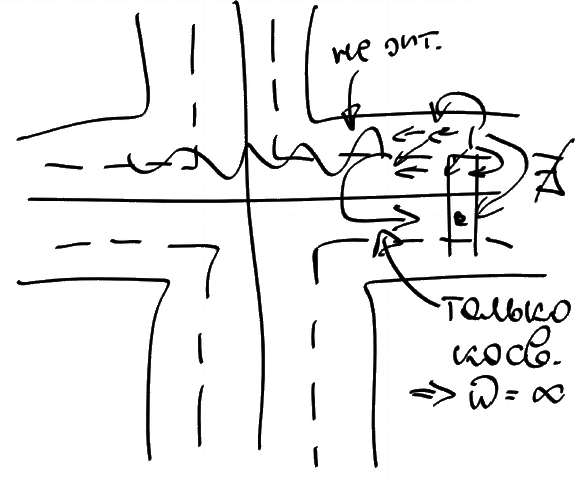
\includegraphics[width=0.6\textwidth]{graphics/pic07.png} 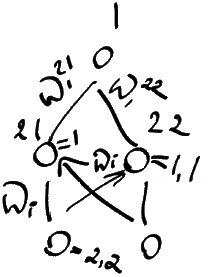
\includegraphics[width=0.2\textwidth]{graphics/pic08.png}

$\omega_ij$ — вес перехода.

$\omega_1^{21} \leq \omega_1^{22}$

$\sum \omega \rightarrow min$

$i : \exists(i - j)$

Алгоритм Дейкстры — нахождение оптимального маршрута в графе.

Характеристики $r_i$:
\begin{enumerate}
    \item Длина ($l$)
    \item Качество ($q$)
    \item Ограничения скорости ($V_{max}$)
\end{enumerate}

$\omega = f(l, V_{max}, q)$

Время: $\left.f(\omega, \{E\}, r_0, r_T) \rightarrow min\right|\Rightarrow V_{\text{ср}} = \dfrac{\sum \dfrac{\sum l}{T}}{N} \Rightarrow T_\text{ср} \Rightarrow Q_i^{end}$

\section*{Ещё более сложная ситуация}

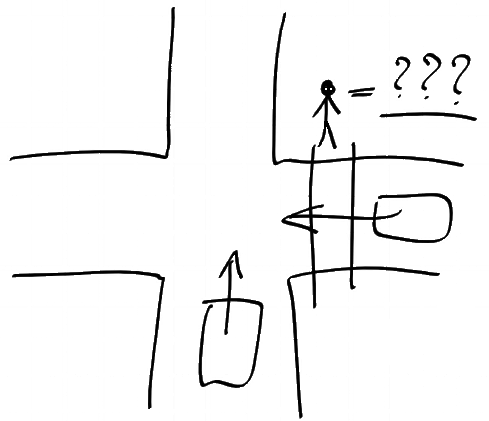
\includegraphics[width=0.6\textwidth]{graphics/pic09.png}

$R = R_{const} \cup R_{dynamic} \cup R_{zero}$. $R$ — риски. $R_{const}$ — известные проблемы (e.g. пешеходные переходы). Решается логикой. $R_dynamic$ — динамические проблемы. Решается сенсорами и предсказанием поведения.

ACAS — стандарт полёта самолётов (управления полётами). Есть $h$ допустимая, к которой стремимся. Разлёт с конфликтующим самолётом должен происходить в рамках одного $r$. Решить задачу алгоритмом Дейкстры по причине роста графа экспоненциально при росте вариантов движения невозможно в оперативное время.

ITS — intellectual transport system — самообучающиеся светофоры.

Модель полицейских участков.

Ad-hoc добавление навигаторов автомобилей.

Полицейский делится на 2 части:
\begin{itemize}
    \item Общение с другими полицейскими
    \item Общение с машинами
\end{itemize}
\end{document}